\documentclass{beamer}

\usetheme{metropolis}
\usecolortheme{default}
\usepackage{ragged2e}
\title{ACHIEVO}
\subtitle{A Productivity WebApp}
\institute[Program]{
        \inst{Women Engineers}
        \inst{TalentSprint}
}
\date{22/06/2023}

\begin{document}

\begin{frame}
  \maketitle
\end{frame}

\begin{frame}{Team Members}
    \begin{itemize}
        \item Nidhi Iyer
        \item Khyati Satija
        \item Pankhuri Asthana
        \item Srinayana Mandalapu
        \item Anushka Shankar
    \end{itemize}
\end{frame}

\begin{frame}{Introduction}
    \begin{itemize}
        \item A user-centric web application for productivity.
        \item Addresses procrastination, lack of focus, and planning issues.
    \end{itemize}
\end{frame}

\begin{frame}{Objectives}
    \begin{itemize}
        \item To enhance our learning.
        \item To explore various technologies via the process.
        \item To gain insights into how such features work.
        \item To implement our learnings and knowledge into our web-app.
        \item To deploy it and provide a solution to the raised issue.
    \end{itemize}
\end{frame}

\begin{frame}{Approach}
    \begin{itemize}
        \item Collaborative Work: Divided tasks evenly among team members.
        \item User-Centric Design: Prioritize understanding user needs and preferences.
        \item Frontend-First: Focus on frontend development initially.
        \item Backend Development: Implement core functionalities and data storage.
        \item Iterative Development: Continuously refine and enhance based on feedback.
    \end{itemize}
\end{frame}

\begin{frame}{Tech Stack}
    \begin{figure}
        \begin{minipage}[t]{0.2\textwidth}
            \centering
            \includegraphics[width=\textwidth]{frontend.jpeg}
            \caption{Frontend}
        \end{minipage}\hfill
        \begin{minipage}[t]{0.2\textwidth}
            \centering
            \includegraphics[width=\textwidth]{node.js_backend.png}
            \caption{Backend}
        \end{minipage}\hfill
        \begin{minipage}[t]{0.2\textwidth}
            \centering
            \includegraphics[width=\textwidth]{mongoDB.png}
            \caption{Database}
        \end{minipage}\hfill
        \begin{minipage}[t]{0.2\textwidth}
            \centering
            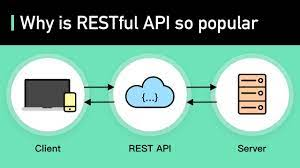
\includegraphics[width=\textwidth]{API.jpeg}
            \caption{RESTful APIs}
        \end{minipage}\hfill
    \end{figure}
\end{frame}

\begin{frame}{Challenges and Learnings}
    \textbf{Challenges}
    \begin{enumerate}
        \item Finding it hard to implement what we learnt and taking excess time to figure stuff out.
        \item Lacking in time management.
        \item Implementation of ideas was harder than imagined.
    \end{enumerate}
    \textbf{Learnings}
    \begin{enumerate}
        \item Team and project management.
        \item Making a website using frontend UI and UX.
        \item Breaking things down into smaller parts makes implementation easy.
    \end{enumerate}
\end{frame}

\begin{frame}{Future Scope}
    \begin{itemize}
        \item Complete the UI/UX according to the theme decided, improve responsiveness and animation.
        \item Build the remaining features.
        \item Finalise the logo.
        \item Learn and understand backend and API functioning.
        \item Work on deployment.
        \item Conduct user testing and gather feedback for further improvements.
    \end{itemize}
\end{frame}

\begin{frame}{Conclusion}
    \justifying
    Hence, Let's ACHIEVO \\
    \bigskip
    \textbf{Domain: } Web Development \\
    \textbf{Status: } Ideation \\
    \bigskip
    \Huge\textbf{Thank You !}
\end{frame}

\end{document}

